\documentclass[aspectratio=169,10pt]{beamer}

\usetheme{default}
\usefonttheme{professionalfonts}
\usepackage[T1]{fontenc}
\usepackage[utf8]{inputenc}
\usepackage{lmodern}
\usepackage{amsmath,amssymb,bm}
\usepackage{graphicx}
\usepackage{booktabs,array,tabularx}
\usepackage{tikz}
\usetikzlibrary{arrows.meta,positioning,calc,decorations.pathreplacing,shapes.geometric}
\usepackage{hyperref}

\hypersetup{colorlinks=true,urlcolor=blue!60!black,citecolor=blue!60!black,linkcolor=blue!60!black}
\definecolor{ink}{RGB}{24,39,58}
\definecolor{blue}{RGB}{35,105,170}
\definecolor{teal}{RGB}{22,126,122}
\definecolor{orange}{RGB}{220,111,31}
\definecolor{red}{RGB}{190,55,55}
\definecolor{softblue}{RGB}{235,244,252}
\definecolor{softteal}{RGB}{231,246,242}
\definecolor{softorange}{RGB}{255,243,227}
\definecolor{softred}{RGB}{252,236,236}

\setbeamercolor{normal text}{fg=ink,bg=white}
\setbeamercolor{structure}{fg=blue}
\setbeamercolor{frametitle}{fg=ink,bg=white}
\setbeamercolor{title}{fg=ink}
\setbeamercolor{subtitle}{fg=blue}
\setbeamercolor{block title}{fg=white,bg=blue}
\setbeamercolor{block body}{fg=ink,bg=softblue}
\setbeamercolor{alerted text}{fg=red}
\setbeamertemplate{navigation symbols}{}
\setbeamertemplate{itemize item}{\color{blue}\small$\blacktriangleright$}
\setbeamertemplate{itemize subitem}{\color{teal}\scriptsize$\blacktriangleright$}
\setbeamertemplate{footline}{\hfill\color{blue!60!black}\scriptsize\insertframenumber~/~\inserttotalframenumber\hspace{1.2em}\vspace{0.65em}}
\setbeamertemplate{frametitle}{\vspace{0.35em}\hspace{0.25em}\insertframetitle\par\vspace{0.12em}\color{blue!25}\rule{\textwidth}{0.6pt}}
\setbeamerfont{block title}{size=\small}
\setlength{\parskip}{0.18em}
\setlength{\tabcolsep}{3pt}
\renewcommand{\arraystretch}{1.16}
\newcolumntype{Y}{>{\raggedright\arraybackslash}X}

\newcommand{\citep}[1]{\textcolor{blue!70!black}{\scriptsize[\cite{#1}]}}
\newcommand{\source}[1]{\par\vspace{0.15em}{\tiny\color{blue!55!black}\raggedright #1\par}}
\newcommand{\figref}[1]{\par\vspace{0.12em}{\tiny\color{blue!60!black}\raggedright\textit{Figure source: }#1\par}}
\newcommand{\key}[1]{\textcolor{teal!80!black}{\textbf{#1}}}
\newcommand{\warn}[1]{\textcolor{red!80!black}{\textbf{#1}}}

\title{From local Maxwell to mesoscopic response}
\subtitle{Literature results, model hierarchy, and a close reading of paper [1]}
\author{Journal club | critical literature study}
\institute{Based on the supplied Structured Mesoscopic Optical Response Review (2026)}
\date{23 July 2026}

\begin{document}

\documentclass[aspectratio=169,10pt]{beamer}

\usetheme{default}
\usefonttheme{professionalfonts}
\usepackage[T1]{fontenc}
\usepackage[utf8]{inputenc}
\usepackage{lmodern}
\usepackage{amsmath,amssymb,bm}
\usepackage{graphicx}
\usepackage{booktabs,array,tabularx}
\usepackage{tikz}
\usetikzlibrary{arrows.meta,positioning,calc,decorations.pathreplacing,shapes.geometric}
\usepackage{hyperref}

\hypersetup{colorlinks=true,urlcolor=blue!60!black,citecolor=blue!60!black,linkcolor=blue!60!black}
\definecolor{ink}{RGB}{24,39,58}
\definecolor{blue}{RGB}{35,105,170}
\definecolor{teal}{RGB}{22,126,122}
\definecolor{orange}{RGB}{220,111,31}
\definecolor{red}{RGB}{190,55,55}
\definecolor{softblue}{RGB}{235,244,252}
\definecolor{softteal}{RGB}{231,246,242}
\definecolor{softorange}{RGB}{255,243,227}
\definecolor{softred}{RGB}{252,236,236}

\setbeamercolor{normal text}{fg=ink,bg=white}
\setbeamercolor{structure}{fg=blue}
\setbeamercolor{frametitle}{fg=ink,bg=white}
\setbeamercolor{title}{fg=ink}
\setbeamercolor{subtitle}{fg=blue}
\setbeamercolor{block title}{fg=white,bg=blue}
\setbeamercolor{block body}{fg=ink,bg=softblue}
\setbeamercolor{alerted text}{fg=red}
\setbeamertemplate{navigation symbols}{}
\setbeamertemplate{itemize item}{\color{blue}\small$\blacktriangleright$}
\setbeamertemplate{itemize subitem}{\color{teal}\scriptsize$\blacktriangleright$}
\setbeamertemplate{footline}{\hfill\color{blue!60!black}\scriptsize\insertframenumber~/~\inserttotalframenumber\hspace{1.2em}\vspace{0.65em}}
\setbeamertemplate{frametitle}{\vspace{0.35em}\hspace{0.25em}\insertframetitle\par\vspace{0.12em}\color{blue!25}\rule{\textwidth}{0.6pt}}
\setbeamerfont{block title}{size=\small}
\setlength{\parskip}{0.18em}
\setlength{\tabcolsep}{3pt}
\renewcommand{\arraystretch}{1.16}
\newcolumntype{Y}{>{\raggedright\arraybackslash}X}

\newcommand{\citep}[1]{\textcolor{blue!70!black}{\scriptsize[\cite{#1}]}}
\newcommand{\source}[1]{\par\vspace{0.15em}{\tiny\color{blue!55!black}\raggedright #1\par}}
\newcommand{\figref}[1]{\par\vspace{0.12em}{\tiny\color{blue!60!black}\raggedright\textit{Figure source: }#1\par}}
\newcommand{\key}[1]{\textcolor{teal!80!black}{\textbf{#1}}}
\newcommand{\warn}[1]{\textcolor{red!80!black}{\textbf{#1}}}

\title{From local Maxwell to mesoscopic response}
\subtitle{Literature results, model hierarchy, and a close reading of paper [1]}
\author{Journal club | critical literature study}
\institute{Based on the supplied Structured Mesoscopic Optical Response Review (2026)}
\date{23 July 2026}

\begin{document}

\begin{frame}[plain]
  \vspace{0.5em}
  {\usebeamerfont{title}\color{ink}\Huge\bfseries From local Maxwell\\[0.12em] to mesoscopic response\par}
  \vspace{0.4em}
  {\usebeamerfont{subtitle}\color{blue}\Large Literature evidence and a close reading of paper [1]\par}
  \vfill
  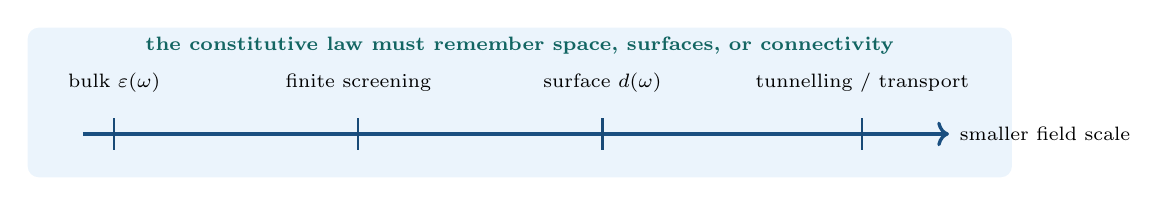
\begin{tikzpicture}[x=1cm,y=1cm]
    \fill[softblue,rounded corners=4pt] (0,0) rectangle (12.5,1.9);
    \draw[blue!75!black,very thick,->] (0.7,0.55)--(11.7,0.55) node[right,black,font=\scriptsize]{smaller field scale};
    \foreach \x/\lab in {1.1/{bulk $\varepsilon(\omega)$},4.2/{finite screening},7.3/{surface $d(\omega)$},10.6/{tunnelling / transport}}{
      \draw[blue!70!black,thick] (\x,0.35)--(\x,0.75);
      \node[align=center,font=\scriptsize] at (\x,1.2){\lab};
    }
    \node[font=\scriptsize\bfseries,teal!80!black] at (6.25,1.67){the constitutive law must remember space, surfaces, or connectivity};
  \end{tikzpicture}
  \vfill
  {\large\color{ink}A literature-led critical analysis, not a chronological paper summary.\par}
  \vspace{0.25em}
  {\scriptsize\color{blue!65!black}Main evidence: 2009--2026; historical anchors: Bennett/Lang--Kohn (1970) and Feibelman (1982).\par}
\end{frame}

\begin{frame}{Talk structure: evidence before interpretation}
\begin{columns}[T,onlytextwidth]
  \column{0.48\textwidth}
  \begin{block}{What the guidelines require}
    \begin{enumerate}
      \item Motivation and scientific question
      \item Background and competing approaches
      \item Methods, controls, and artifacts
      \item Key literature results
      \item Critical analysis and alternative explanations
      \item Weaknesses, open questions, conclusions
    \end{enumerate}
  \end{block}
  \column{0.48\textwidth}
  \begin{alertblock}{The rule used on every data slide}
    Separate three statements:
    \begin{enumerate}
      \item what is directly measured or computed;
      \item what the authors infer;
      \item what another mechanism could imitate.
    \end{enumerate}
  \end{alertblock}
  \vspace{0.3em}
  \begin{block}{My standard for a strong claim}
    The same parameter set should explain a reactive observable and a dissipative or transport observable.
  \end{block}
\end{columns}
\source{Structure follows the supplied Journal Club Guidelines, Talk Template, and Short Checklist.}
\end{frame}

\begin{frame}{Central question and answer in one slide}
\begin{columns}[T,onlytextwidth]
  \column{0.49\textwidth}
  \begin{block}{Scientific question}
    How far can a nanostructure be scaled before bulk local $\varepsilon(\omega)$, a sharp interface, and classical Maxwell boundary conditions stop being predictive? Which response object should replace them?
  \end{block}
  \vspace{0.25em}
  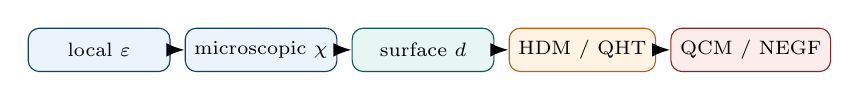
\begin{tikzpicture}[node distance=0.28cm and 0.18cm, every node/.style={font=\scriptsize,align=center}]
    \node[draw=blue!60!black,fill=softblue,rounded corners,minimum width=1.8cm,minimum height=0.55cm] (a){local $\varepsilon$};
    \node[draw=blue!60!black,fill=softblue,rounded corners,minimum width=1.8cm,minimum height=0.55cm,right=of a] (b){microscopic $\chi$};
    \node[draw=teal!70!black,fill=softteal,rounded corners,minimum width=1.8cm,minimum height=0.55cm,right=of b] (c){surface $d$};
    \node[draw=orange!85!black,fill=softorange,rounded corners,minimum width=1.8cm,minimum height=0.55cm,right=of c] (d){HDM / QHT};
    \node[draw=red!70!black,fill=softred,rounded corners,minimum width=1.8cm,minimum height=0.55cm,right=of d] (e){QCM / NEGF};
    \foreach \x/\y in {a/b,b/c,c/d,d/e}{\draw[-{Latex},thick] (\x)--(\y);}
  \end{tikzpicture}
  \column{0.46\textwidth}
  \begin{alertblock}{Short answer}
    These are not rival ``quantum corrections.'' They retain different pieces of the same two-point response and have different domains of validity.
  \end{alertblock}
  \begin{itemize}
    \item $d_\perp,d_\parallel$ compress the interface.
    \item HDM/QHT retains continuum density/current dynamics.
    \item TDDFT/NEGF is the reference when atoms or charge transfer matter.
  \end{itemize}
\end{columns}
\end{frame}

\begin{frame}{Local response is a sharp-interface approximation}
\begin{columns}[T,onlytextwidth]
  \column{0.48\textwidth}
  \begin{block}{What LRA keeps}
    \begin{align*}
      \mathbf P(\mathbf r,\omega)&=\varepsilon_0\chi(\omega)\mathbf E(\mathbf r,\omega),\\
      \mathbf J(\mathbf r,\omega)&=\sigma(\omega)\mathbf E(\mathbf r,\omega),\\
      \varepsilon_m(\omega)&=\varepsilon_\infty-\frac{\omega_p^2}{\omega(\omega+i\gamma)}.
    \end{align*}
    Geometry, radiation, absorption, and bulk dispersion can be treated accurately by Mie, BEM, FEM, or FDTD.
  \end{block}
  \column{0.47\textwidth}
  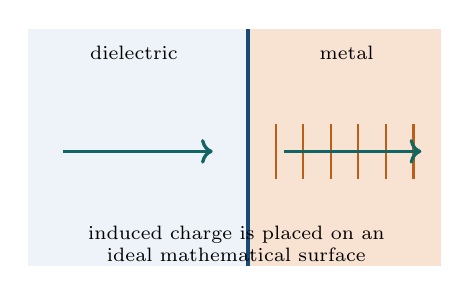
\begin{tikzpicture}[x=1cm,y=1cm]
    \fill[blue!8] (0,0) rectangle (5.25,3.0);
    \fill[orange!20] (2.8,0) rectangle (5.25,3.0);
    \draw[very thick,blue!70!black] (2.8,0)--(2.8,3.0);
    \node[font=\scriptsize] at (1.35,2.7){dielectric};
    \node[font=\scriptsize] at (4.05,2.7){metal};
    \foreach \x in {3.15,3.5,3.85,4.2,4.55,4.9}{\draw[orange!85!black,thick] (\x,1.1)--(\x,1.8);}
    \node[font=\scriptsize,align=center,text width=4.6cm] at (2.65,0.28){induced charge is placed on an ideal mathematical surface};
    \draw[teal!80!black,very thick,->] (0.45,1.45)--(2.35,1.45);
    \draw[teal!80!black,very thick,->] (3.25,1.45)--(5.0,1.45);
  \end{tikzpicture}
  \begin{alertblock}{What LRA discards}
    Spatial dispersion $\varepsilon(\mathbf k,\omega)$, diffuse equilibrium density, finite charge centroids, atomistic transitions, and tunnel conductivity.
  \end{alertblock}
\end{columns}
\source{Classical platform: Mie \citep{mie1908}; local graphene sheet starting point: Jablan et al. \citep{jablan2009}.}
\end{frame}

\begin{frame}{The smallest feature controls the breakdown}
\begin{columns}[T,onlytextwidth]
  \column{0.50\textwidth}
  \begin{block}{Scale comparisons}
    \[
      q\ell,\qquad \frac{\ell}{R},\qquad \frac{\ell}{g},\qquad \frac{\ell}{t}
    \]
    Here $\ell$ may be a screening length, spill-out width, Fermi wavelength, mean free path, tunnelling decay length, or exciton coherence radius.
  \end{block}
  \begin{itemize}
    \item A $100\,$nm antenna with a $1\,$nm gap contains $q\sim 1/g$ components.
    \item A large isolated particle can be less nonlocal than a smaller, strongly coupled gap.
    \item Mesh refinement improves the solution of LRA; it does not change the constitutive law.
  \end{itemize}
  \column{0.46\textwidth}
  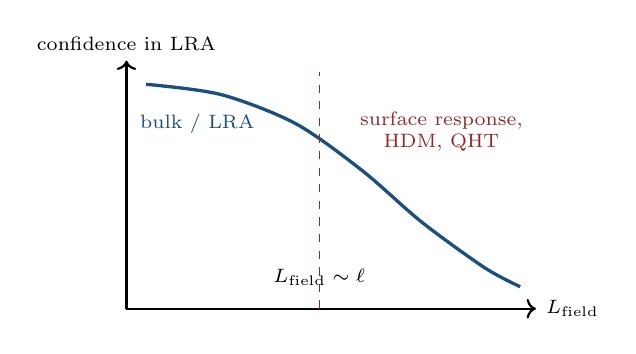
\begin{tikzpicture}[x=1cm,y=1cm]
    \draw[->,thick] (0,0)--(5.2,0) node[right,font=\scriptsize]{$L_\mathrm{field}$};
    \draw[->,thick] (0,0)--(0,3.15) node[above,font=\scriptsize]{confidence in LRA};
    \draw[blue!75!black,very thick] plot[smooth] coordinates{(0.25,2.85)(1.2,2.72)(2.15,2.35)(3.0,1.75)(3.75,1.1)(4.55,0.52)(5.0,0.28)};
    \draw[dashed,red!75!black] (2.45,0)--(2.45,3.0);
    \node[font=\scriptsize,align=center,text width=1.8cm,blue!75!black] at (0.9,2.35){bulk / LRA};
    \node[font=\scriptsize,align=center,text width=2.3cm,red!75!black] at (4.0,2.25){surface response, HDM, QHT};
    \node[font=\scriptsize] at (2.45,0.4){$L_\mathrm{field}\sim\ell$};
  \end{tikzpicture}
\end{columns}
\source{Thresholds are indicative and material/geometry dependent; see the supplied review's validity criterion.}
\end{frame}

\begin{frame}{Literature map: the main evidence chain}
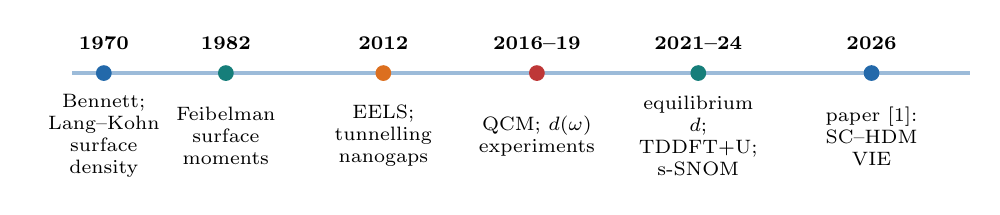
\begin{tikzpicture}[x=1cm,y=1cm]
  \draw[blue!45,very thick] (0.6,1.9)--(12.0,1.9);
  \foreach \x/\yr/\txt/\col in {1.0/1970/{Bennett; Lang--Kohn\\surface density}/blue,2.55/1982/{Feibelman\\surface moments}/teal,4.55/2012/{EELS; tunnelling\\nanogaps}/orange,6.5/2016--19/{QCM; $d(\omega)$\\experiments}/red,8.55/2021--24/{equilibrium $d$;\\TDDFT+U; s-SNOM}/teal,10.75/2026/{paper [1]:\\SC--HDM VIE}/blue}{
    \fill[\col] (\x,1.9) circle (0.1);
    \node[font=\scriptsize\bfseries,align=center] at (\x,2.28){\yr};
    \node[font=\scriptsize,align=center,text width=1.7cm] at (\x,1.1){\txt};
  }
\end{tikzpicture}
\vspace{0.4em}
\begin{columns}[T,onlytextwidth]
  \column{0.31\textwidth}
  \begin{block}{Microscopic evidence}
    Size-dependent EELS and TDDFT show that a fixed bulk $\varepsilon$ misses atomistic structure and discrete transitions.
  \end{block}
  \column{0.31\textwidth}
  \begin{block}{Mesoscopic evidence}
    Complex interface response and complex gap-mode propagation measure both phase and loss.
  \end{block}
  \column{0.31\textwidth}
  \begin{block}{Computational bridge}
    Paper [1] makes diffuse SC--HDM cheap for a sphere and exposes its limitations.
  \end{block}
\end{columns}
\source{Selected primary literature from the review: \citep{bennett1970,langkohn1970,feibelman1982,scholl2012,zhu2016,mortensen2021,chaudhary2024,mystilidis2026}.}
\end{frame}

\begin{frame}{Literature result 1: size-dependent particle plasmons}
\begin{columns}[T,onlytextwidth]
  \column{0.59\textwidth}
  
\includegraphics[width=\linewidth,height=0.70\textheight,keepaspectratio]{assets/chaudhary2024_fig3.png}
  \figref{M. Chaudhary and H.-C. Weissker, Nature Communications 15, 9225 (2024), Fig. 3, “Optical spectra of silver clusters and nanoparticles from 4 to 923 atoms,” DOI: 10.1038/s41467-024-53428-6. Open-access article.}
  \column{0.37\textwidth}
  \begin{block}{Direct result}
    The LSPR energy changes systematically with inverse radius. The calculation spans Ag$_4$ to Ag$_{923}$, approximately a 3-nm particle.
  \end{block}
  \begin{itemize}
    \item Small clusters show discrete electron--hole structure.
    \item Larger clusters develop a broad collective resonance.
    \item Shape matters: icosahedral and fcc-based clusters of similar size do not coincide.
  \end{itemize}
  \begin{alertblock}{Critical reading}
    Size-dependent shifts are evidence against a fixed bulk local $\varepsilon$, but they combine quantum confinement, atomistic shape, and $d$-electron screening.
  \end{alertblock}
\end{columns}
\end{frame}

\begin{frame}{Literature result 2: microscopic spectra connect atoms to plasmons}
\begin{columns}[T,onlytextwidth]
  \column{0.58\textwidth}
  
\includegraphics[width=\linewidth,height=0.68\textheight,keepaspectratio]{assets/chaudhary2024_fig2.png}
  \figref{Chaudhary and Weissker (2024), Nature Communications 15, 9225, Fig. 2, DOI: 10.1038/s41467-024-53428-6. Open-access article.}
  \column{0.37\textwidth}
  \begin{block}{Why this is a benchmark}
    RT--TDDFT+$U$ retains atomic geometry and filled $d$-shell screening, then recovers the crossover from discrete spectra to broad LSPRs.
  \end{block}
  \begin{itemize}
    \item Agreement with experiment across the size range is a genuine validation of the electronic model.
    \item The effective $U$ is used consistently from small clusters to bulk-like silver.
    \item The result sets a scale: even $\sim10^4$ active electrons is still only about 3 nm.
  \end{itemize}
  \begin{alertblock}{Role in the hierarchy}
    Use microscopic spectra as a calibration/reference, then transfer validated response information to mesoscopic solvers.
  \end{alertblock}
\end{columns}
\end{frame}

\begin{frame}{Literature result 3: nonlocal screening precedes tunnelling}
\begin{columns}[T,onlytextwidth]
  \column{0.59\textwidth}
  
\includegraphics[width=\linewidth,height=0.68\textheight,keepaspectratio]{assets/zhu2016_fig1.jpg}
  \figref{W. Zhu et al., Nature Communications 7, 11495 (2016), Fig. 1, DOI: 10.1038/ncomms11495. Open-access article.}
  \column{0.37\textwidth}
  \begin{block}{Regime sequence}
    \begin{enumerate}
      \item Large gaps: local Maxwell with empirical $\varepsilon_M$.
      \item Few-nm gaps: screening charges shift by $\delta_F$; the optical gap differs from the geometric gap.
      \item Sub-nm gaps: optical tunnelling changes the boundary topology and charge-transfer plasmons appear before contact.
    \end{enumerate}
  \end{block}
  \begin{alertblock}{Model consequence}
    Surface response or HDM can describe separated bodies. Once the gap conducts, use QCM calibrated to TDDFT/NEGF or explicit transport.
  \end{alertblock}
\end{columns}
\end{frame}

\begin{frame}{Literature result 4: optics must be paired with conductance}
\begin{columns}[T,onlytextwidth]
  \column{0.31\textwidth}
  \begin{block}{Capacitive gap}
    \centering
    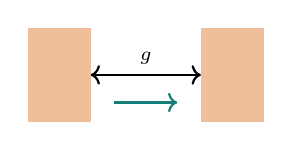
\begin{tikzpicture}[x=1cm,y=1cm]
      \fill[orange!45] (0,0) rectangle (0.8,1.2);\fill[orange!45] (2.2,0) rectangle (3.0,1.2);
      \draw[<->,thick] (0.8,0.6)--(2.2,0.6) node[midway,above,font=\scriptsize]{$g$};
      \draw[teal,thick,->] (1.1,0.25)--(1.9,0.25);
    \end{tikzpicture}
    \smallskip
    Bonding dimer plasmon redshifts as $g$ shrinks.
  \end{block}
  \column{0.31\textwidth}
  \begin{block}{Tunnelling onset}
    \centering
    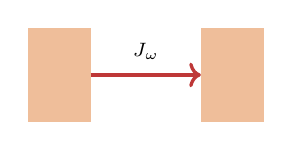
\begin{tikzpicture}[x=1cm,y=1cm]
      \fill[orange!45] (0,0) rectangle (0.8,1.2);\fill[orange!45] (2.2,0) rectangle (3.0,1.2);
      \draw[red,very thick,->] (0.8,0.6)--(2.2,0.6);
      \node[font=\scriptsize] at (1.5,0.9){$J_\omega$};
    \end{tikzpicture}
    \smallskip
    Optical crossover tracks junction conductance.
  \end{block}
  \column{0.31\textwidth}
  \begin{block}{Charge-transfer plasmon}
    \centering
    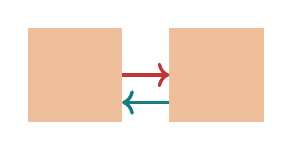
\begin{tikzpicture}[x=1cm,y=1cm]
      \fill[orange!45] (0,0) rectangle (1.2,1.2);\fill[orange!45] (1.8,0) rectangle (3.0,1.2);
      \draw[red,very thick,->] (1.2,0.6)--(1.8,0.6);
      \draw[teal,very thick,->] (1.8,0.25)--(1.2,0.25);
    \end{tikzpicture}
    \smallskip
    The gap is no longer a purely dielectric boundary.
  \end{block}
\end{columns}
\vspace{0.45em}
\begin{block}{Evidence base}
  Savage et al. correlated optical spectra with conductance in a controllable Au junction; Tan et al. showed that molecular conductance controls the capacitive-to-conductive plasmon crossover. These observations are stronger than a nominal gap-distance calibration alone.
\end{block}
\source{K. J. Savage et al., Nature 491, 574--577 (2012), DOI: 10.1038/nature11653; S. F. Tan et al., Science 343, 1496--1499 (2014), DOI: 10.1126/science.1248797.}
\end{frame}

\begin{frame}{Literature result 5: a complex Feibelman response is measurable}
\begin{columns}[T,onlytextwidth]
  \column{0.61\textwidth}
  
\includegraphics[width=\linewidth,height=0.68\textheight,keepaspectratio]{assets/yang2019_fig3_lw685.png}
  \figref{Y. Yang et al., Nature 576, 248--252 (2019), Fig. 3, “A general theoretical and experimental framework for nanoscale electromagnetism,” DOI: 10.1038/s41586-019-1803-1. Figure downloaded from the publisher page for educational journal-club use.}
  \column{0.35\textwidth}
  \begin{block}{What is measured}
    Film-coupled resonators provide families of resonance shifts and linewidths from which the complex Au--AlO$_x$ surface response $d_\perp(\omega)$ is retrieved.
  \end{block}
  \begin{itemize}
    \item The response is dispersive and complex, not one fitted length.
    \item Nonclassical shifts exceed 30\% in the reported architecture.
    \item Causality and Kramers--Kronig consistency matter for broadband retrieval.
  \end{itemize}
  \begin{alertblock}{Critical reading}
    Agreement with both shift and linewidth is much stronger than a fit to one resonance, but transfer still depends on facet, reference plane, and wavevector.
  \end{alertblock}
\end{columns}
\end{frame}

\begin{frame}{Literature result 6: complex gap-mode propagation exposes loss}
\begin{columns}[T,onlytextwidth]
  \column{0.58\textwidth}
  
\includegraphics[width=\linewidth,height=0.70\textheight,keepaspectratio]{assets/boroviks2022_fig4.png}
  \figref{S. Boroviks et al., Nature Communications 13, 3105 (2022), Fig. 4, “Extremely confined gap plasmon modes: when nonlocality matters,” DOI: 10.1038/s41467-022-30737-2. Open-access article.}
  \column{0.38\textwidth}
  \begin{block}{Direct result}
    s-SNOM measures the complex propagation constant of gap surface plasmons in crystalline Au--Al$_2$O$_3$--Au waveguides.
  \end{block}
  \begin{itemize}
    \item The real part tracks confinement.
    \item The imaginary part tracks propagation loss.
    \item Few-nm gaps show excess loss relative to LRA.
    \item GNOR fits the complex trend, but its diffusion constant is an effective closure rather than a unique microscopic observable.
  \end{itemize}
\end{columns}
\end{frame}

\begin{frame}{Equilibrium inhomogeneity is not dynamical nonlocality}
\begin{columns}[T,onlytextwidth]
  \column{0.51\textwidth}
  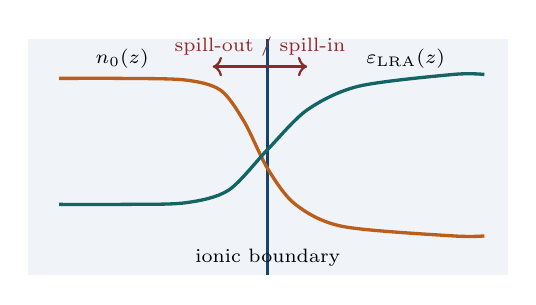
\begin{tikzpicture}[x=1cm,y=1cm]
    \fill[blue!7] (0,0) rectangle (6.1,3.0);
    \draw[very thick,blue!65!black] (3.05,0)--(3.05,3.0);
    \draw[orange!85!black,very thick] plot[smooth] coordinates{(0.4,2.5)(1.2,2.5)(2.0,2.48)(2.45,2.35)(2.75,1.95)(3.05,1.35)(3.4,0.9)(4.0,0.62)(5.4,0.5)(5.8,0.5)};
    \draw[teal!80!black,very thick] plot[smooth] coordinates{(0.4,0.9)(1.2,0.9)(2.0,0.92)(2.55,1.08)(3.05,1.6)(3.55,2.1)(4.2,2.4)(5.4,2.55)(5.8,2.55)};
    \node[font=\scriptsize] at (1.2,2.75){$n_0(z)$};
    \node[font=\scriptsize] at (4.8,2.75){$\varepsilon_\mathrm{LRA}(z)$};
    \node[font=\scriptsize,align=center] at (3.05,0.22){ionic boundary};
    \draw[<->,red!75!black,thick] (2.35,2.65)--(3.55,2.65) node[midway,above,font=\scriptsize]{spill-out / spill-in};
  \end{tikzpicture}
  \column{0.44\textwidth}
  \begin{block}{Result from Mortensen et al. (2021)}
    A smooth equilibrium electron-density profile produces a finite-width induced charge and hence a finite surface-response centroid even when the constitutive law is local pointwise.
  \end{block}
  \begin{alertblock}{Separation of mechanisms}
    Spill-out/spill-in is an equilibrium inhomogeneity. Finite electron-gas compressibility is dynamical nonlocality. They can reinforce or cancel.
  \end{alertblock}
  \begin{itemize}
    \item Useful: explains a finite $d$ without a full TDDFT calculation.
    \item Limited: omits detailed Friedel oscillations, facets, and correlations.
  \end{itemize}
\end{columns}
\source{N. A. Mortensen et al., Nanophotonics 10, 3647--3657 (2021), DOI: 10.1515/nanoph-2021-0084.}
\end{frame}

\begin{frame}{Model hierarchy: what each literature route retains}
\small
\begin{tabularx}{\linewidth}{@{}p{0.16\linewidth}Y Y Y@{}}
\toprule
\textbf{Route} & \textbf{Response object} & \textbf{Retained physics} & \textbf{Main failure mode}\
\midrule
LRA & $\varepsilon(\omega)$ or $\sigma_{2D}(\omega)$ & bulk dispersion, geometry, radiation, absorption & sharp boundary; no $q$ dependence\
TDDFT / RPA / NEGF & $\chi(\mathbf r,\mathbf r';\omega)$ & atoms, transitions, facets, tunnelling, correlations/transport & scale and parameter-sweep cost\
Feibelman response & $d_\perp(\omega),d_\parallel(\omega)$ & charge/current centroids, surface loss & first-order, interface-local, possibly $q$-dependent\
HDM / GNOR & $\varepsilon(\mathbf k,\omega)$ or hydrodynamic fields & compressibility, longitudinal response, effective loss & hard wall or fitted closure; no chemistry\
SC--HDM / QHT & $n_0(\mathbf r)$ plus induced $n_1,\mathbf J$ & diffuse surface plus continuum dynamics & functional, tail, interband calibration\
QCM / transport & conductive gap response & tunnelling and charge-transfer modes & chemistry/transport calibration\
\bottomrule
\end{tabularx}
\source{Synthesis of the review's model hierarchy; primary examples: \citep{feibelman1982,mortensen2014,mortensen2021,esteban2012}.}
\end{frame}

\begin{frame}{Paper [1]: what problem is it actually solving?}
\begin{columns}[T,onlytextwidth]
  \column{0.40\textwidth}
  \begin{block}{Paper [1] in the review}
    \textbf{Mystilidis et al.} develop a volume-integral equation (VIE) formalism for the self-consistent hydrodynamic Drude model (SC--HDM).
  \end{block}
  \begin{itemize}
    \item Target: isolated spherical nanoparticles, $R=1$--$5\,$nm.
    \item Material: sodium-like Drude metal, $\hbar\omega_p=6.04\,$eV.
    \item SC--HDM retains both nonlocal electron dynamics and equilibrium spill-out.
    \item The paper is a computational-method paper, not a new experiment.
  \end{itemize}
  \column{0.57\textwidth}
  
\includegraphics[width=\linewidth,height=0.70\textheight,keepaspectratio]{assets/mystilidis2026_fig1.png}
  \figref{C. Mystilidis, C. Tserkezis, G. A. E. Vandenbosch, N. A. Mortensen, and X. Zheng, Nanophotonics 15(13), e70179 (2026), Fig. 1, DOI: 10.1002/nap2.70179, CC BY 4.0.}
\end{columns}
\end{frame}

\begin{frame}{Paper [1], method: remove the artificial bottleneck}
\begin{columns}[T,onlytextwidth]
  \column{0.48\textwidth}
  \begin{block}{Why differential-equation SC--HDM is costly}
    \begin{itemize}
      \item The density tail extends beyond the ionic radius $R$ to $R+s$.
      \item Matter-wave length scales require a fine mesh.
      \item The exterior electromagnetic domain is physically infinite.
      \item Longitudinal and transverse fields are coupled.
    \end{itemize}
  \end{block}
  \column{0.47\textwidth}
  \begin{block}{What the VIE changes}
    \begin{enumerate}
      \item Use the homogeneous dyadic Green tensor to handle radiation without meshing the exterior.
      \item Expand polarization in vector spherical harmonics.
      \item Use cubic radial Lagrange functions for the diffuse density.
      \item Separate TE, TM, and longitudinal sectors into small radial blocks.
    \end{enumerate}
  \end{block}
  \begin{alertblock}{The key claim}
    For a sphere the coupled three-dimensional multiphysics problem becomes a set of one-dimensional radial problems. The speedup is symmetry-enabled.
  \end{alertblock}
\end{columns}
\source{Paper [1], §§2.1--2.3; Fig. 1 shows the DE-to-IE-to-spherical reduction. Full citation on the previous slide.}
\end{frame}

\begin{frame}{Paper [1], result 1: validation against OpenSANS}
\begin{columns}[T,onlytextwidth]
  \column{0.65\textwidth}
  
\includegraphics[width=\linewidth,height=0.73\textheight,keepaspectratio]{assets/mystilidis2026_fig2.png}
  \figref{Mystilidis et al. (2026), Nanophotonics 15(13), e70179, Fig. 2, DOI: 10.1002/nap2.70179.}
  \column{0.31\textwidth}
  \begin{block}{Directly shown}
    \begin{itemize}
      \item LRA and HDM VIE spectra track OpenSANS S-matrix results.
      \item Reported relative error is about 0.08\% in the benchmark metrics.
      \item The benchmark covers radii $R=1$--$5\,$nm and both LRA and HDM.
      \item The quasistatic trend is recovered for the dipolar LSP.
    \end{itemize}
  \end{block}
  \begin{alertblock}{What this validates}
    The discretization and spherical implementation—not the material realism of SC--HDM.
  \end{alertblock}
\end{columns}
\end{frame}

\begin{frame}{Paper [1], result 2: SC--HDM adds spill-out and a surface mode}
\begin{columns}[T,onlytextwidth]
  \column{0.66\textwidth}
  
\includegraphics[width=\linewidth,height=0.73\textheight,keepaspectratio]{assets/mystilidis2026_fig3.png}
  \figref{Mystilidis et al. (2026), Nanophotonics 15(13), e70179, Fig. 3, DOI: 10.1002/nap2.70179.}
  \column{0.30\textwidth}
  \begin{block}{At $R=2\,$nm}
    \begin{itemize}
      \item LRA dipole: $\approx3.49\,$eV.
      \item HDM dipole: $\approx3.64\,$eV.
      \item SC--HDM dipole: $\approx3.30\,$eV.
      \item Bennett-type feature: near $4.1\,$eV.
      \item Runtime: 85.69, 87.95, 94.36 s for LRA, HDM, SC--HDM.
    \end{itemize}
  \end{block}
  \begin{alertblock}{Physical reading}
    Hard-wall compressibility pushes charge inward; diffuse SC--HDM density shifts response outward. The sign is model dependent.
  \end{alertblock}
\end{columns}
\end{frame}

\begin{frame}{Paper [1], result 3: what the $d_\perp$ extraction means}
\begin{columns}[T,onlytextwidth]
  \column{0.49\textwidth}
  \begin{block}{The paper's interpretation}
    The spherical induced-charge centroid is analogous to a perpendicular Feibelman parameter. It is smooth around the dipole resonance but develops a Lorentzian feature at the Bennett resonance.
  \end{block}
  \begin{itemize}
    \item The Bennett mode corresponds to sign-changing induced charge across the finite-width surface layer.
    \item This suggests a multiscale pipeline: SC--HDM generates a surface response that a cheaper boundary solver can reuse.
    \item The first zero near 4.62 eV is reported as unphysical/numerically sensitive.
  \end{itemize}
  \column{0.47\textwidth}
  \begin{alertblock}{My critical reading}
    A finite-sphere centroid is not automatically a planar, causal, transferable $d(q,\omega)$.
  \end{alertblock}
  \begin{block}{Needed before transfer}
    \begin{enumerate}
      \item convergence with spill-out allowance $s$ and radial mesh;
      \item comparison with planar TDDFT for the same material;
      \item facet, environment, and reference-plane dependence;
      \item causality/passivity checks over a broadband range;
      \item sensitivity to the orbital-free functional.
    \end{enumerate}
  \end{block}
\end{columns}
\source{Paper [1], Fig. 3(b,e) and discussion in §3.2; the review explicitly warns that the extracted curve is not yet a universal sodium $d$ parameter.}
\end{frame}

\begin{frame}{Paper [1], contribution versus unresolved boundary}
\begin{columns}[T,onlytextwidth]
  \column{0.47\textwidth}
  \begin{block}{Established by paper [1]}
    \begin{itemize}
      \item A VIE with spherical symmetry reproduces known LRA/HDM benchmarks.
      \item SC--HDM can be solved with about 10\% overhead over LRA in the tested geometry.
      \item Diffuse equilibrium density changes resonance positions and creates a Bennett-type feature.
      \item The implementation can extract a mesoscopic surface-response quantity.
    \end{itemize}
  \end{block}
  \column{0.47\textwidth}
  \begin{alertblock}{Still open}
    \begin{itemize}
      \item arbitrary 3D shapes, edges, substrates, and touching junctions;
      \item real noble metals with interband screening and facets;
      \item stable, causal $d(q,\omega)$ for transfer to BEM/FEM;
      \item systematic functional and spill-out-tail calibration;
      \item direct experimental validation of the sodium spectra.
    \end{itemize}
  \end{alertblock}
\end{columns}
\vspace{0.35em}
\begin{block}{Verdict}
  Paper [1] is a strong solver contribution and a useful mesoscopic bridge. Its spectra are a sodium-like numerical benchmark, not yet a universal material response.
\end{block}
\end{frame}

\begin{frame}{Literature comparison: what is actually constrained?}
\small
\begin{tabularx}{\linewidth}{@{}p{0.21\linewidth}Y Y@{}}
\toprule
\textbf{Study / observable} & \textbf{What it constrains} & \textbf{What remains degenerate}\
\midrule
Scholl 2012: individual-particle EELS & fixed bulk local $\varepsilon$ is insufficient for few-nm Ag particles & size, shape, surface, and quantum transitions\
Savage 2012; Tan 2014: optics + conductance & optical crossover follows conductive coupling across a gap & chemistry and junction geometry still matter\
Yang 2019: shift + linewidth families & complex Au--AlO$_x$ surface response is measurable & facet, reference plane, and $q$ dependence\
Boroviks 2022: complex gap $q$ & few-nm confinement adds propagation loss beyond LRA & GNOR parameter is an effective closure\
Chaudhary 2024: TDDFT+$U$ spectra & atomistic structure and $d$-shell physics connect clusters to LSPRs & computational scale and functional transfer\
Mystilidis 2026 [1]: VIE SC--HDM & diffuse continuum response can be computed cheaply for spheres & arbitrary geometry and material validation\
\bottomrule
\end{tabularx}
\source{Primary sources: \citep{scholl2012,savage2012,tan2014,yang2019,boroviks2022,chaudhary2024,mystilidis2026}.}
\end{frame}

\begin{frame}{A practical model-selection workflow}
\begin{columns}[T,onlytextwidth]
  \column{0.23\textwidth}
  \begin{block}{1. Scale}
    Find $g$, curvature $R$, film thickness $t$, and modal $q$.
  \end{block}
  \begin{block}{2. Baseline}
    Constrain $\varepsilon$, geometry, roughness, facet, spacer, and uncertainty.
  \end{block}
  \column{0.23\textwidth}
  \begin{block}{3. Observable}
    Is the discrepancy a shift, loss, phase, transport signal, or several at once?
  \end{block}
  \begin{block}{4. Boundary}
    Does charge remain confined? If not, a polarizable surface is incomplete.
  \end{block}
  \column{0.23\textwidth}
  \begin{block}{5. Model}
    Use $d$/HDM/QHT for separated bodies; QCM/NEGF/TDDFT for conductive gaps.
  \end{block}
  \begin{block}{6. Transfer}
    Check facet, reference plane, curvature, $q$ dependence, passivity, and causality.
  \end{block}
  \column{0.23\textwidth}
  \begin{alertblock}{7. Validate}
    Require two observables and, where possible, a microscopic benchmark.
  \end{alertblock}
  \begin{block}{For 2D hybrids}
    Keep metal $d$ response separate from $\sigma_{2D}(q,\omega)$ or $\chi_{2D}(q,\omega)$.
  \end{block}
\end{columns}
\source{Condensed from the supplied review, §7.4.}
\end{frame}

\begin{frame}{A metal--2D hybrid contains two nonlocal subsystems}
\begin{columns}[T,onlytextwidth]
  \column{0.47\textwidth}
  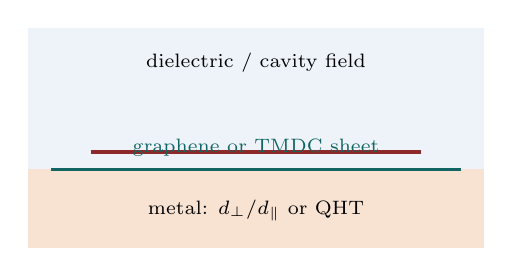
\begin{tikzpicture}[x=1cm,y=1cm]
    \fill[blue!8] (0,1.0) rectangle (5.8,2.8);
    \fill[orange!20] (0,0) rectangle (5.8,1.0);
    \draw[teal!80!black,very thick] (0.3,1.0)--(5.5,1.0);
    \draw[red!75!black,very thick] (0.8,1.22)--(5.0,1.22);
    \node[font=\scriptsize] at (2.9,2.35){dielectric / cavity field};
    \node[font=\scriptsize,teal!80!black] at (2.9,1.28){graphene or TMDC sheet};
    \node[font=\scriptsize] at (2.9,0.48){metal: $d_\perp/d_\parallel$ or QHT};
  \end{tikzpicture}
  \column{0.48\textwidth}
  \begin{tabularx}{\linewidth}{@{}p{0.30\linewidth}Y@{}}
    \toprule
    \textbf{Subsystem} & \textbf{Response object}\
    \midrule
    metal surface & $d_\perp(\omega),d_\parallel(\omega)$ or $d(q,\omega)$\
    graphene & $\sigma_{2D}(q,\omega)$\
    TMDC exciton & $\chi_{2D}(q,\omega)$, often BSE/polariton informed\
    cavity & Maxwell Green tensor and geometry\
    \bottomrule
  \end{tabularx}
  \vspace{0.35em}
  \begin{alertblock}{Do not hide both in one effective $\varepsilon$}
    Otherwise momentum dependence and loss are assigned to the wrong subsystem, and the model cannot say what experiment would discriminate them.
  \end{alertblock}
\end{columns}
\source{Graphene/TMDC context: \citep{lundeberg2017,alpeggiani2018,nerl2024,kleemann2017}.}
\end{frame}

\begin{frame}{Conclusions: the critical verdict}
\begin{enumerate}
  \item \key{Local Maxwell remains the zeroth-order theory.} Its validity is controlled by the smallest field scale compared with electronic lengths.
  \item \key{Literature experiments show distinct failure modes.} EELS probes size/atomistic effects; conductance-linked optics probes tunnelling; complex $d$ and complex $q$ probe interface response and loss.
  \item \key{Surface response and hydrodynamics are complementary.} $d$ compresses an interface; QHT retains continuum density/current dynamics.
  \item \key{Paper [1] makes a real computational contribution.} The spherical VIE reduces SC--HDM overhead to about 10\%, validates against OpenSANS, and produces a Bennett response—but does not yet establish transferability.
  \item \key{The next experiment must be overdetermined.} Pair resonance energy with linewidth/phase, conductance, or a microscopic benchmark.
\end{enumerate}
\vspace{0.4em}
\begin{alertblock}{Open boundary}
  At the angstrom conductive junction, surface polarization, atomic chemistry, and quantum transport become inseparable.
\end{alertblock}
\end{frame}

\begin{frame}{Discussion questions}
\begin{block}{Questions to take to the journal club}
  \begin{enumerate}
    \item Which of the literature experiments most cleanly separates a reactive correction from a dissipative one?
    \item Is the SC--HDM functional in paper [1] a useful calibration model for noble metals, or mainly a solver benchmark?
    \item What convergence test would you demand first for the extracted $d_\perp$: radial mesh, spill-out allowance, functional, or geometry?
    \item Can one transfer a finite-sphere centroid to a planar interface without explicitly checking $q$ dependence?
    \item For a real nanogap, when would you switch from $d$/HDM/QHT to QCM, NEGF, or TDDFT?
  \end{enumerate}
\end{block}
\vfill
\centering\large\color{blue!80!black}The key question is not “is it quantum?” but “which response object has the missing physics?”
\end{frame}

\appendix
\begin{frame}{Source trace: review pages used to audit paper [1]}
\begin{columns}[T,onlytextwidth]
  \column{0.49\textwidth}
  
\includegraphics[width=\linewidth,height=0.70\textheight,keepaspectratio]{assets/review_anchor_page12.png}
  \source{Rendered from the supplied review PDF, p. 12: VIE design choices, validation, 2-nm energies, and runtimes.}
  \column{0.49\textwidth}
  
\includegraphics[width=\linewidth,height=0.70\textheight,keepaspectratio]{assets/review_anchor_page13.png}
  \source{Rendered from the supplied review PDF, p. 13: $d_\perp$ extraction, limitations, and contribution/open-problem split.}
\end{columns}
\end{frame}

\begin{frame}[allowframebreaks]{Selected references}
\scriptsize
\bibliographystyle{unsrt}
\bibliography{references}
\end{frame}

\end{document}

\end{document}
